\documentclass[11pt]{article}
\usepackage{graphicx,natbib,amsmath,color,matlab-prettifier,listings,epstopdf}
\makeatletter
\renewcommand{\maketitle}{
\begin{center}

\pagestyle{empty}
\phantom{.}  %necessary to add space on top before the title
\vspace{3cm}

{\Huge \bf \@title\par}
\vspace{2.5cm}

{\LARGE Deniz Dilan Dogan}\\[1cm]

{\Large\@date}

\vspace{4.5cm}

School of Science and Engineering\\
University of Dundee
%if you want something in the bottom of the page just use \vfill before that.

\end{center}
}\makeatother
\title{SEIR Modelling COVID-19 to Analyse Government Strategies in the UK}
\author{Deniz Dilan Dogan}
\begin{document}
	\maketitle

\newpage
	\tableofcontents
\pagebreak
\section{Abstract}
Since March 2020, when The World Health Organization officially acknowledged the outbreak of COVID-19 as a pandemic, every country has put in efforts to form strategies to contain said pandemic. By data we can see how effective these strategies are, but what if they were used from day $1$ of the pandemic? This study aims to analyse then compare the main strategies used by the UK government. To then find the ideal strategy or the ideal combination of strategies to contain the COVID-19 pandemic. Comparing relative to a no-policy environment, we can observe if there is a need for strategies to begin with. Then considering the NHS capacity we can conclude if the strategy was successful at avoiding a healthcare crisis, which is the most crucial part of defining a good strategy in this piece. \par
These comparisons via observation of graphs made using the SEIR model, corresponding to the no-policy environment and each strategy. Separately plotting hospitalisations, ICU cases with their respective thresholds in terms of hospital beds available. \par
The results show that strategies are necessary to contain the COVID-19 pandemic, with the hospitalisations in the no-policy environment significantly greater than every other strategy. The ideal strategy is given by vaccinations, but to implement said strategy we need time to develop vaccinations which can be bought by other strategies.

\section{Introduction and Overview}
\subsection{Introduction to pandemic}
During late December of 2019 Wuhan Municipal Health Commission, reported to the World Health Organization a series of pneumonia cases, all in which the causal agent was unknown. The number of patients which had adjacent symptoms had become sufficiently significant for WHO to investigate this report further using information collected from authorities in Wuhan. Soon after, China publicised the genetic sequence of COVID-19, known as the novel coronavirus at the time. This was immediately followed by the inevitable first recorded case outside of China which occurred during mid-January in Thailand. The patient had been travelling from Wuhan, combining this new case with information gathered from the first cluster of patients, strongly implied human-to-human transmission, in turn WHO acknowledged that there was a potential for an outbreak. After months of analysing data, strategising with experts globally, devising plans and support systems to contain the virus, the cases had increased exponentially. On the 11th of March, with over 118,000 cases globally and 4,291 resulting fatalities, WHO announced that COVID-19 fulfilled the required criteria to be classed as a pandemic\citep{WHO'stimelineofCOVID-19}. \par
Since this date the UK government has implemented various strategies to contain the virus. But how effective were/are these strategies if effective at all? The aim of this piece is to analyse and compare strategies used by the UK Government during the current global pandemic of COVID-19, using the SEIR model to determine how lockdowns and general government guidelines have affected fatalities and general transmission of COVID-19. By using MATLAB to model different strategies, with the basis of the code from Nadanomics\citep{MODEL}, we can explore the significance of these strategies in terms of containing the pandemic, in turn the validity of statements made by officials and by the general public.
\subsection{Why modelling of a pandemic is necessary}
Modelling infectious diseases is highly important to the point of necessity as it is the gateway to forecasting how diseases will spread. Just like weather forecasting, modelling diseases allows people to live accordingly and plan accordingly to an outbreak. To respond to a new outbreak, we need to know the severity of the said outbreak i.e., how quickly it is spreading, and how quickly it will spread. If we had no way of measuring the severity of an outbreak, we would have trouble identifying a pandemic to begin with, and we would struggle to find the most appropriate course of action to contain the pandemic. Hence, we would have to react to all outbreaks in the same way for the sake of consistency, which is unsustainable socially and economically. Given some strategies limit our freedom to socialise and contribute to the economy, and on a national scale this could be devastating. \par
An early example of compartmental modelling being used to control a pandemic is given by the work of Sir Ronald Ross in 1902 on the transmission of malaria between mosquitos and humans. He concluded that reducing the population of mosquitos below a critical level can contain the spread of malaria, since it’s extremely hard to control the population of mosquitos this could not be applied for all populations but in the cases where it was applicable, it worked as the model predicted which in turn lead to his Nobel Prize in Medicine\citep{brauer2019introduction}. It is important to note mathematical models are not perfect, they have a set of limitations that are created due to assumptions that are made to simplify the model; to make it accessible. Although, as shown by Sir Ronald Ross’ work, they tend to make good predictions that can help us contain outbreaks.
\section{The Model}
\subsection{Why use this variant of SIR modelling}
This model is appropriate for the COVID-19 pandemic as it allows consideration of the latency period, which is the period between contracting the infection, becoming infectious and the incubation period which is the period between becoming infectious then showing symptoms. The latency period and the incubation period combined is the lag between contact of susceptible and infectious, and consequent infection followed  by symptoms. This lag is represented by the exposed category. The potential to spread when symptoms have not been present yet is extremely low, to the point of insignificance i.e., the showing of symptoms naturally greatly increases the risk of spread\citep{ spreadofCOVID-19}, hence there is no transmission in this lag period that is considered in my models i.e., there is no chance of infection due to contact of susceptible and exposed which will be further outlined in the assumptions of this model. Since this model is with respect to time and the lag between infection and symptoms is sufficiently large\citep{10.1093/cid/ciab746} it is important to reflect this in the model to predict the spread as accurately as possible. \par
If the exposed category was not implemented in these models, we would observe peaks for different categories at a much earlier day during the pandemic. Which would not affect the comparisons but will affect the overall accuracy of the model, which is as crucial to the conclusions of this project, considering the analysis of strategies will factor in the day of peak infections, hospital patients, and ICU patients.
\subsection{Assumptions}
\begin{enumerate}
\item The population stays constant i.e., the death rate and birth rate are approximately equivalent.
\item Every individual is in the exposed category for the same fixed length of time, i.e., infected people will not be infectious with symptoms until 5.8 days\citep{10.1093/cid/ciab746}.
\item All individuals are equally susceptible to COVID-19, and the whole population is considered susceptible at the start of the pandemic.
\item Individuals that are recovered cannot be reinfected i.e., immunity is assumed.
\item There is no heterogeneity between individuals i.e., this model ignores network differences between individuals. 
\item The majority of the population lives in accordance to government guidelines.
\item Population of the UK is equally distributed i.e., population structure is uniform.
\item The rate of transmission of COVID-19 is fixed for each 'strategy'.
\item The removal rate is constant and does not depend on strategy used.
\item People are infectious with symptoms for 7 days\citep{he2020temporal}.
\item Hospital patients are 'removed' from hospital in 8.4 days\citep{vekaria2021hospital}.
\item ICU patients are 'removed' from critical care in 12.4 days\citep{vekaria2021hospital}. 
\item Exposed people cannot spread COVID-19.
\end{enumerate}
\subsection{Variables}
$S$: Number of people susceptible to COVID-19 in the UK.
\newline $E$: Number of people exposed to COVID-19 in the UK.
\newline $I$: Number of people infectious with COVID-19 with symptoms in the UK.
\newline $H$: Number of non-ICU hospital patients with COVID-19 in the UK.
\newline $H_{ICU}$: Number of ICU patients with COVID-19 in the UK.
\newline $R$: Number of people removed by COVID-19 i.e. deceased or recovered in the UK.\par
The variables $I$, $H$ and $H_{ICU}$ split the infectious category into three and are important when defining a good strategy. For this project, I have defined a good strategy as one that controls hospitalisations such that the number of people in hospital does not go over NHS capacity. This capacity is given by the number of hospital beds available in the UK\citep{HBEDS}. There is a different number of beds available for ICU patients as they require more sophisticated medical equipment for treatment, hence why hospitalisations are split into to two categories. If hospitalisations due to COVID-19 go over the capacity or even close to the capacity, people receiving treatment for other diseases will be in danger of delayed treatment whether this be surgery or check-ups that could make the difference between life and death. My models do not consider population structure by assumption $7$, therefore the true peak(s) will be less than predicted by my model. With this in mind, when analysing the models take them as the worst-case models.
\subsection{Parameters}
$ \alpha_1$: Rate of transmission of COVID-19 to susceptible by infectious people.
\newline $ \alpha_2$: Rate of transmission of COVID-19 to susceptible by non-ICU hospital patients.
\newline$ \alpha_3$: Rate of transmission of COVID-19 to susceptible by ICU patients.
\newline$ \beta$: Rate of transition of exposed to infectious.
\newline $ \gamma_1 $: Rate of transition of infectious people to non-ICU patients.
\newline $ \gamma_2 $: Rate of admissions to ICU.
\newline $ \delta_1$: Rate of removal of infectious people.
\newline $ \delta_2$: Rate of removal of non-ICU hospital patients.
\newline $ \delta_3$: Rate of removal of ICU patients. \par
\subsection{System of differential equations}
\begin{equation}
\begin{aligned}
\frac{dS}{dt}&=- \alpha_1 SI - \alpha_2 SH - \alpha_3 SH_{ICU} \\
\frac{dE}{dt}&= \alpha_1 SI + \alpha_2 SH + \alpha_3 SH_{ICU} - \beta E \\
\frac{dI}{dt}&= \beta E -\gamma_1 I -\delta_1 I \\
\frac{dH}{dt}&= \gamma_1 I - \gamma_2 H -\delta_2 H \\
\frac{dH_{ICU}}{dt}&= \gamma_2 H -\delta_3 H_{ICU} \\
\frac{dR}{dt}&=\delta_1 I + \delta_2 H + \delta_3 H_{ICU} \\
\end{aligned}
\end{equation} 
\subsection{Flowchart of the system}
\begin{center}
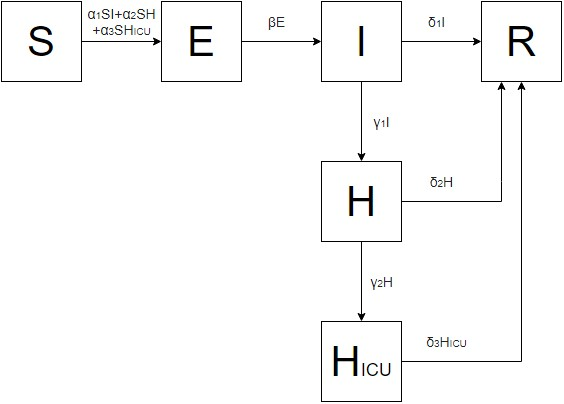
\includegraphics[width=1\textwidth]{SEIHR.jpg} 
\end{center}

\subsection{Calculating parameters using data}
Data used will be taken from the median day of the given strategy, for the no-policy environment, data will be taken from the start of pandemic. For the vaccination environment, four months into vaccinations but using the same $R_0$ number from no-policy environment as we assume that this is the only strategy in play, and does not reduce contact between people in the population. \par
$\alpha_1$, $\alpha_2$, $\alpha_3$ are calculated using the reproductive number given by the data source, the population of the UK and the duration of sickness in days. They are all doubled in value considering that although the whole population is susceptible at the start this decreases very quickly as people are infected, also considering one person does not have potential to spread to the whole population. By assumption $10$, one is infectious with symptoms for 7 days before removal which gives: $\alpha_1=\frac{2R_0}{7N}$. By assumption $11$, one is hospitalised for $8.4$ days before removal which gives: $\alpha_2=\frac{2R_0}{8.4N}$. Finally, by assumption $12$ one is hospitalised in the ICU for $12.4$ days before removal which gives: $\alpha_3=\frac{2R_0}{12.4N}$ where N is the population of the UK and $R_0$ varies depending on the environment. \par
$\beta$ is calculated using assumption $2$, since these models are with respect to time, the unit of time being days and everyone in the exposed category enters the infectious with symptoms category in 5.8 days: $\beta=\frac{1}{5.8}$ for all environments. \par
In the same way $\delta_1$, $\delta_2$, $\delta_3$ are calculated using the duration of stay in days in given category. By assumption $10$: $\delta_1=\frac{1}{7}$, by assumption $11$: $\delta_2=\frac{1}{8.4}$, and by assumption $12$: $\delta_3=\frac{1}{12.4}$. \par
$\gamma_1$ and $\gamma_2$ are calculated using data on admissions to the hospital and the ICU. For $\gamma_1$, the daily hospital admissions over the ongoing cases, and for $\gamma_2$, the daily ICU admissions over the current hospital cases since one cannot go from $I$ directly to $H_{ICU}$. To put it simply, it is the proportion of daily admissions into hospital and ICU.
\subsection{Why the R number is problematic}
The basic reproductive number, $R_0$, generally defined as ‘the average number of secondary cases resulting from a standard primary case in a population that is susceptible entirely’ has implied assumptions. To quantify such an important concept, these implied assumptions are necessary to simplify calculations in turn, to make it as accessible to the general population to use as a reference to understand the severity of the spread. The implied assumptions stem from the fact that this value is an average, more specifically average transmissibility between individuals and the average infections caused by the individual. Ironically, this ignores the definition of an individual, as it generalises the individual. Hence, disregards the existence of heterogeneity in the population. This heterogeneity is intrinsic to the spread of COVID-19 as factors such as social networks and super spreaders\citep{ Reich2020.04.30.20081828} are significant exacerbators of this spread.
There are many methods to calculate $R_0$, most of produce different values for $R_0$ i.e., values that are inconsistent with each other\citep{breban2007theory}, the main one the general public has been exposed to is calculated using existing contact tracing data to estimate spread\citep{R0calculationBBC}, meaning that it is continuously changing and only applies to the recent past, this is also the reproductive number given by the data used to calculate parameters in my models. This heavily relies on data being up to date and accurate, as strategies are planned around the severity of an outbreak. Unfortunately, this type of calculation of $R_0$ does not allow government to plan for what is to come, it helps deal with the current severity.
$R_0$ is commonly used as a threshold for determining whether an outbreak will progress into a pandemic. Where $R_0>1$ implies that the outbreak will progress into a pandemic and in contrast, $R_0<1$ implies outbreak will be contained. \par
However, there are examples of cases where a disease is contained while $R_0>1$, similarly there are cases where disease persists into an outbreak while $R_0<1$\citep{li2011failure}. In turn using the basic reproductive number as a threshold without further evidence that it holds as a threshold is extremely risky. All the caveats surrounding the calculation of $R_0$ i.e., method of calculation and assumptions the model requires to make the calculation of $R_0$ must be carefully considered\citep{li2011failure}. Many diseases are dependent on factors yet to be applied to models we have access to today. The basic reproductive number has many limitations, but currently it is the best tool to measure the severity of an outbreak and the effectiveness of strategies applied to control an outbreak.
\section{Modelling the no-policy environment}
\subsection{Overall no-policy environment}
\begin{center}
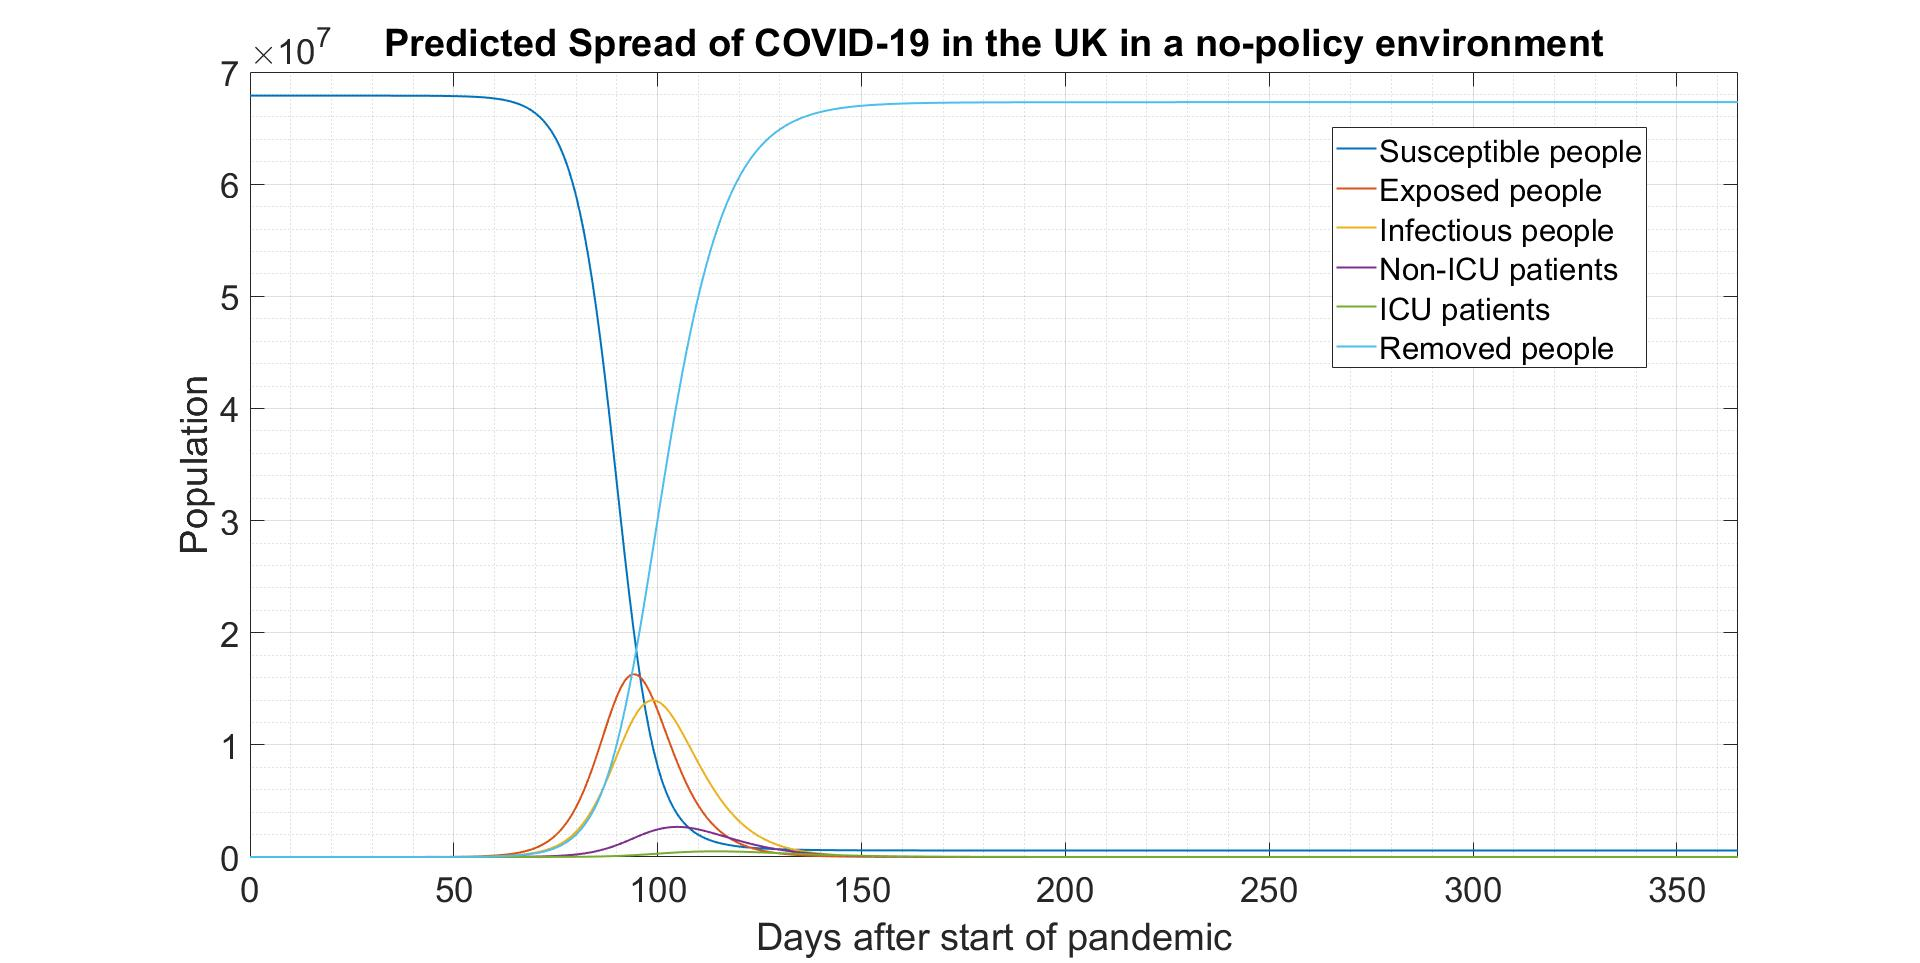
\includegraphics[width=1\textwidth]{No-policySEIHR.jpg} 
\end{center}
Parameters: $R_0=2.4$, $\alpha_1=\frac{2R_0}{7N}$, $\alpha_2=\frac{2R_0}{8.4N}$, $\alpha_3=\frac{2R_0}{12.4N}$, $\gamma_1=\frac{15546-13875}{44399}$, $\gamma_2=\frac{2120-1813}{15546}$ where N is the population of the UK. The peak of infections occurs on day $99$ of the pandemic with $I=13983000$ \par
The endemic occurs when $\frac{dI}{dt}=0$, this is at the peak of infections, given the nature of the one peak model, after this point $\frac{dI}{dt}<0$ hence infections only decrease by day $99$. However, the end of all infections occurs on day $270$ with $S=581600$ and $R=67310000$, R being the number of people immune at the end of all infections.
\subsection{Hospitalisations in a no-policy environment}
\begin{center}
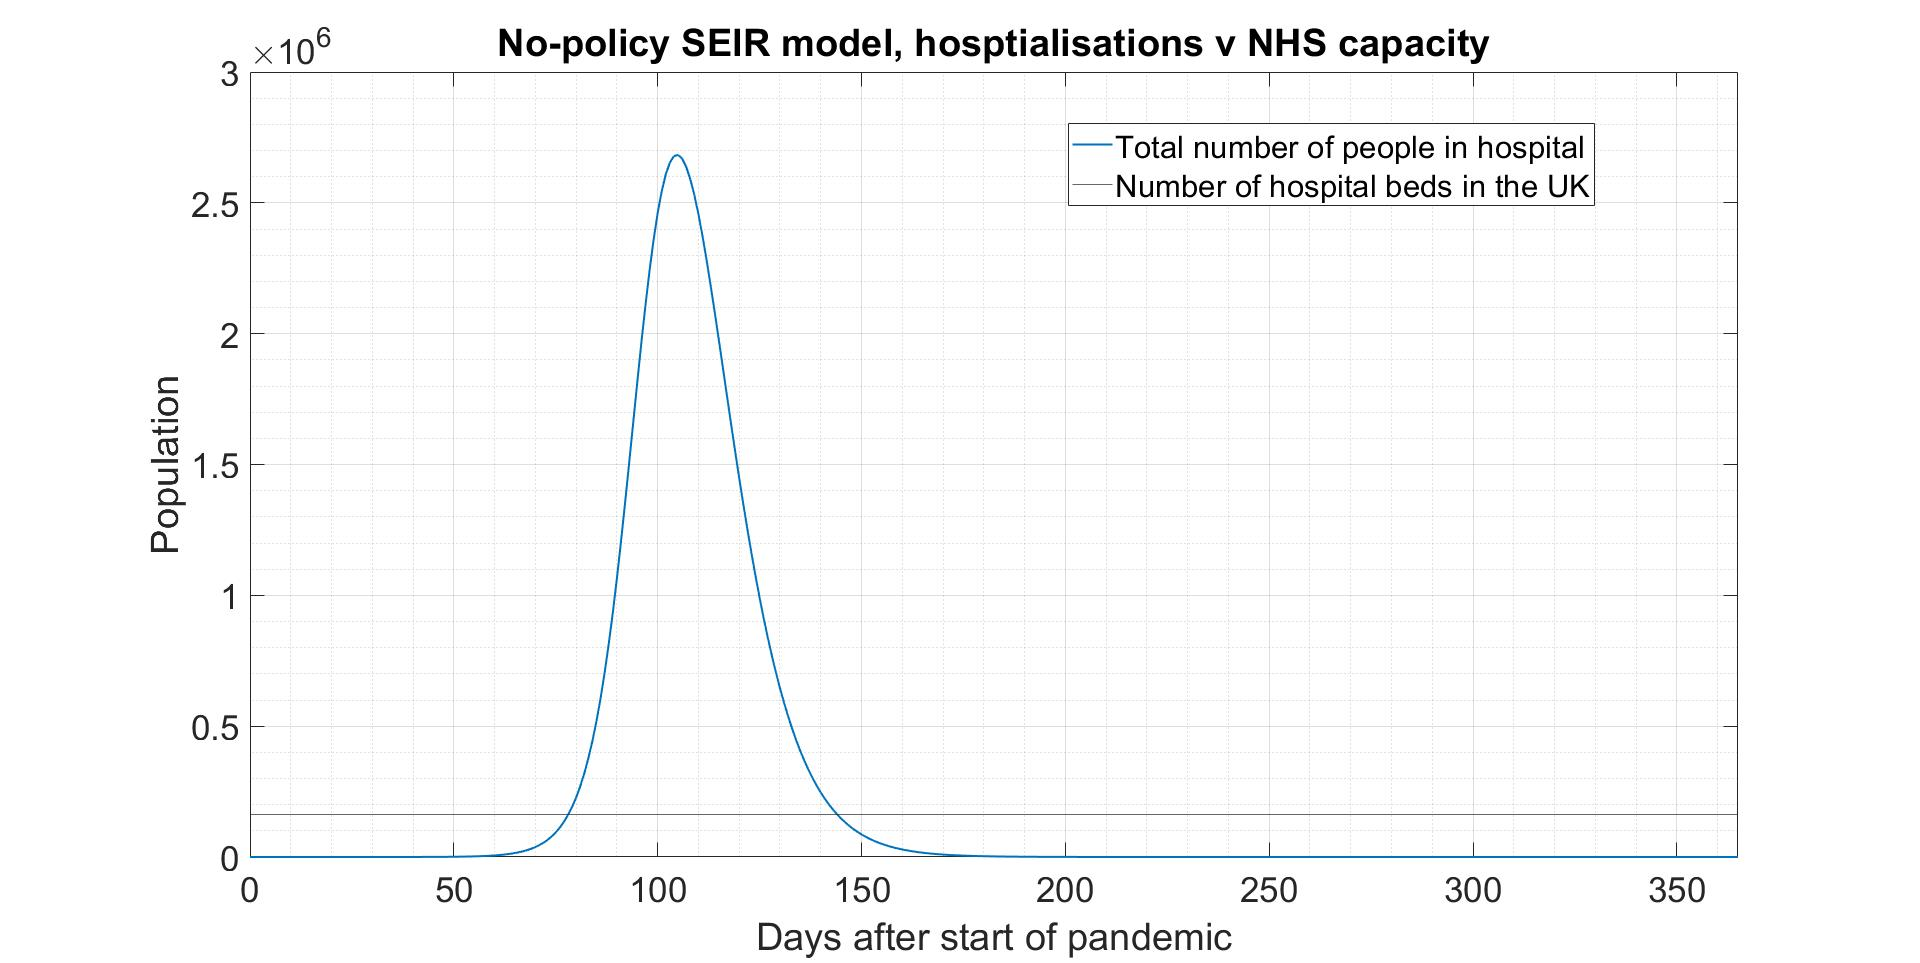
\includegraphics[width=1\textwidth]{No-policyH.jpg} 
\end{center}
\begin{center}
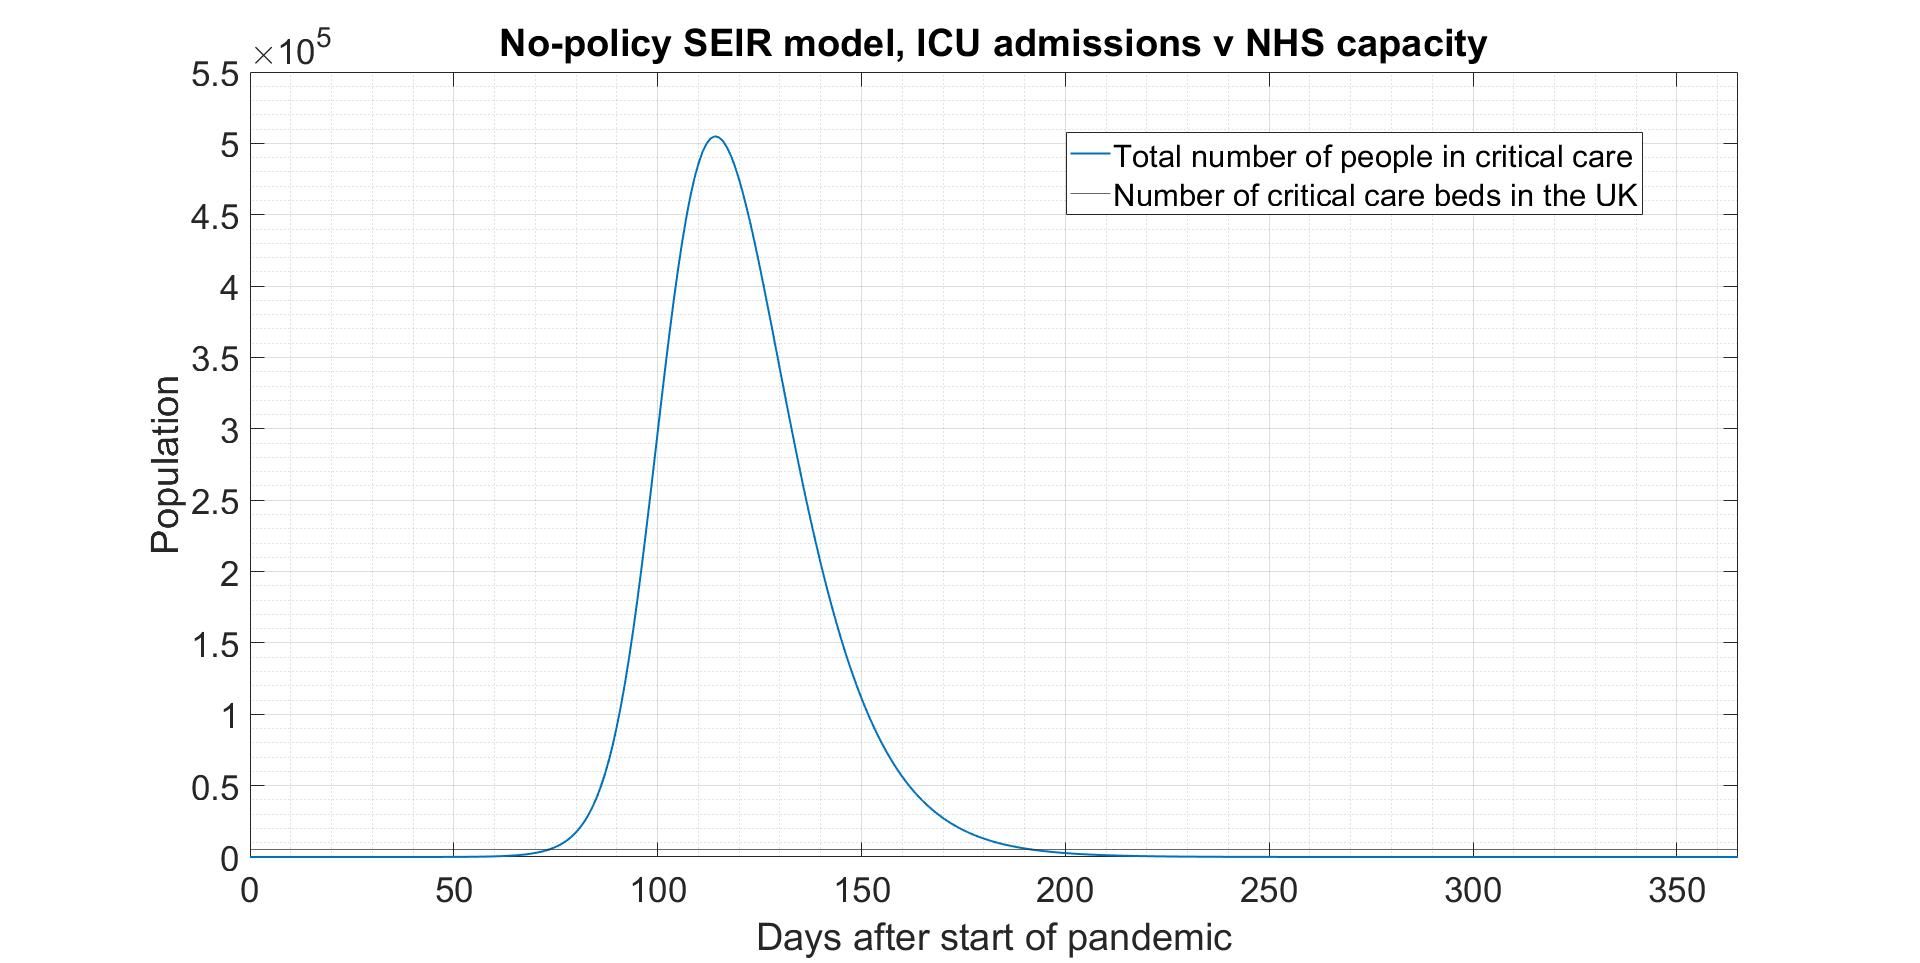
\includegraphics[width=1\textwidth]{No-policyHICU.jpg} 
\end{center}
The peak of ICU patients occurs on day $114$ with $H_{ICU}=504947$, and the peak of hospitalisations occurs on day $105$ of the pandemic with $H=2683170$. The hospitalisations are over capacity from day $78$ to day $144$, for $66$ days, with peak over capacity when there are $2520234$ more hospitalised people than beds available. The ICU is over capacity from day $74$ to day $191$, which is $117$ over capacity, peak over capacity when there are $499991$ more people in the ICU than critical care beds available.
\section{Modelling Strategies}
\subsection{Full Lockdown}
\begin{center}
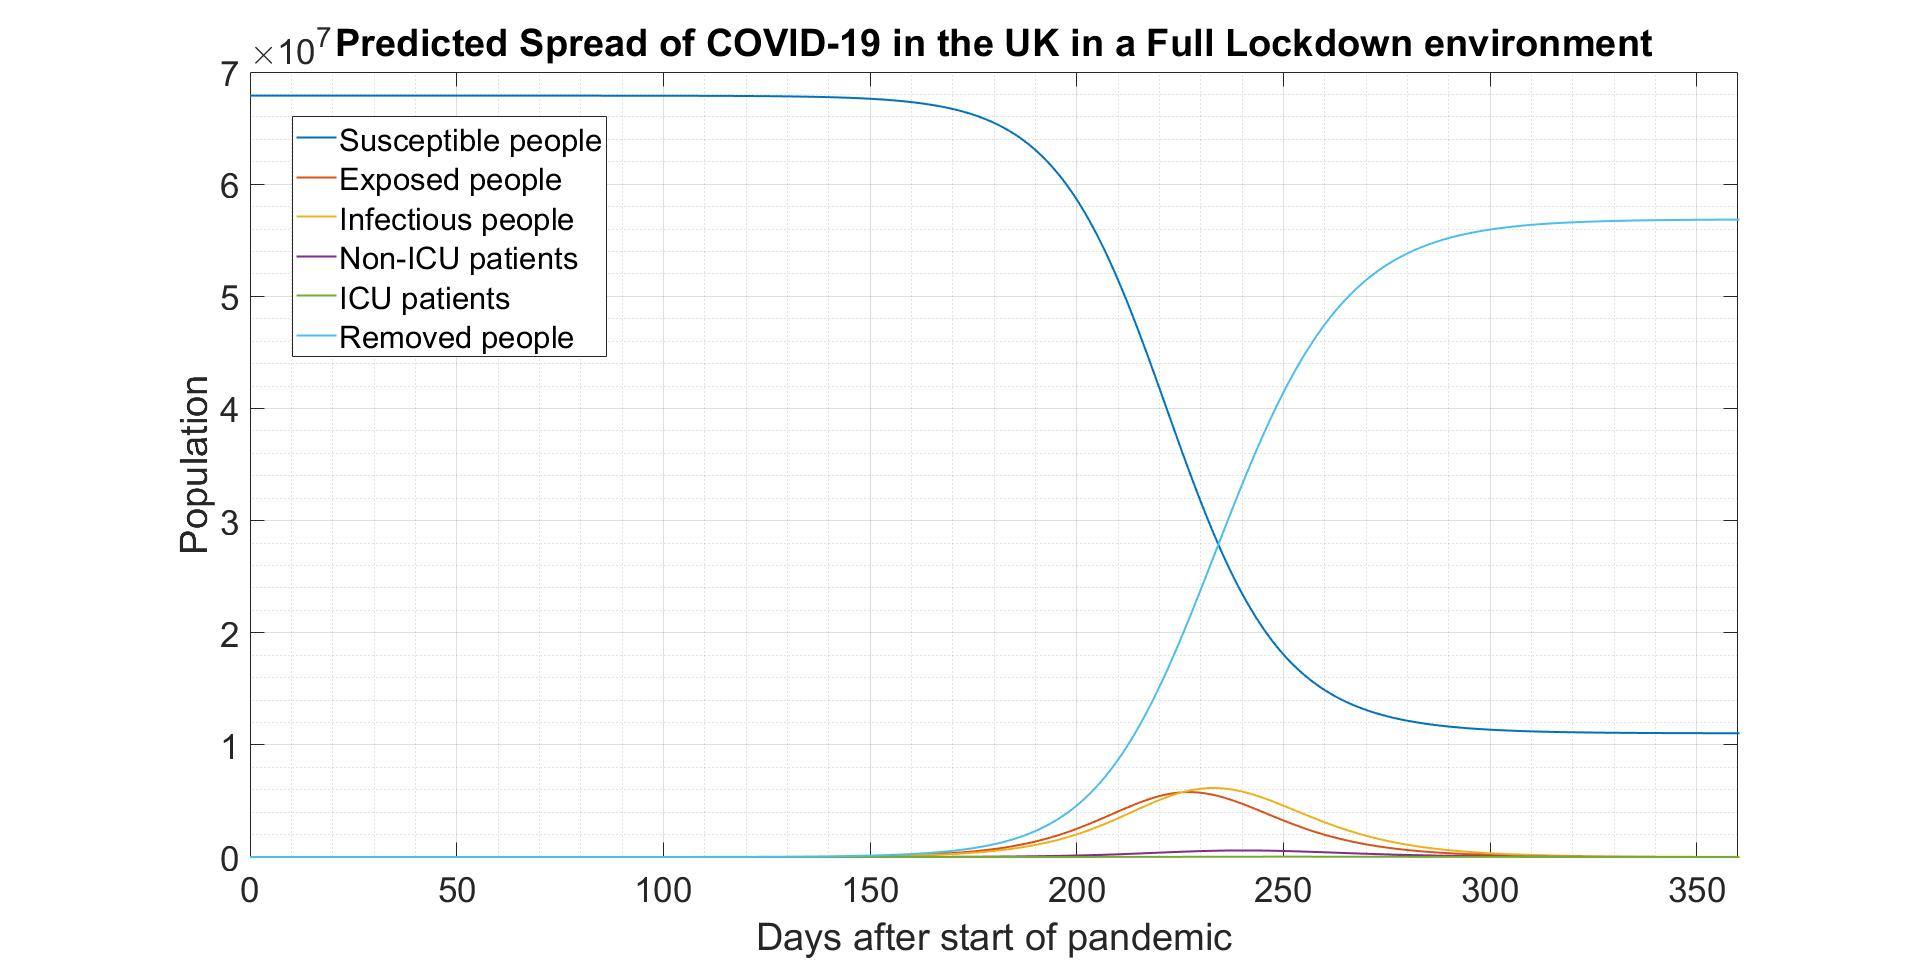
\includegraphics[width=1\textwidth]{FLSEIHR.jpg} 

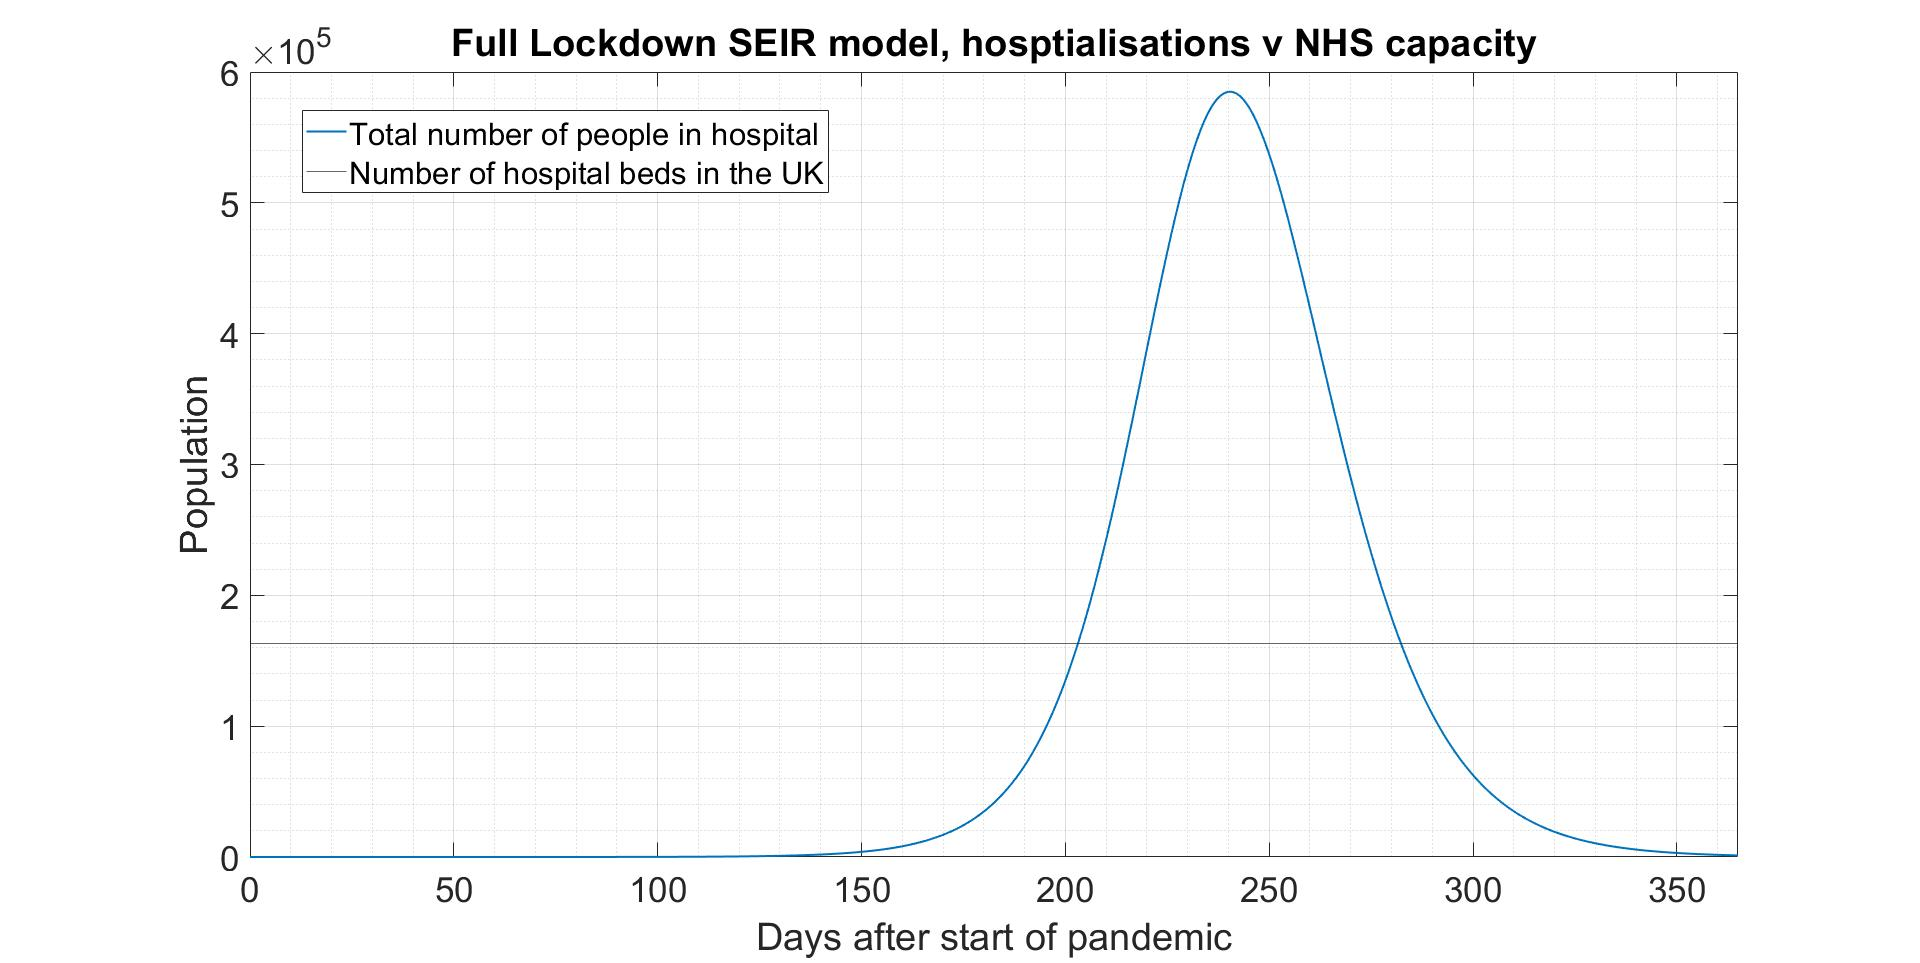
\includegraphics[width=1\textwidth]{FLH.jpg} 

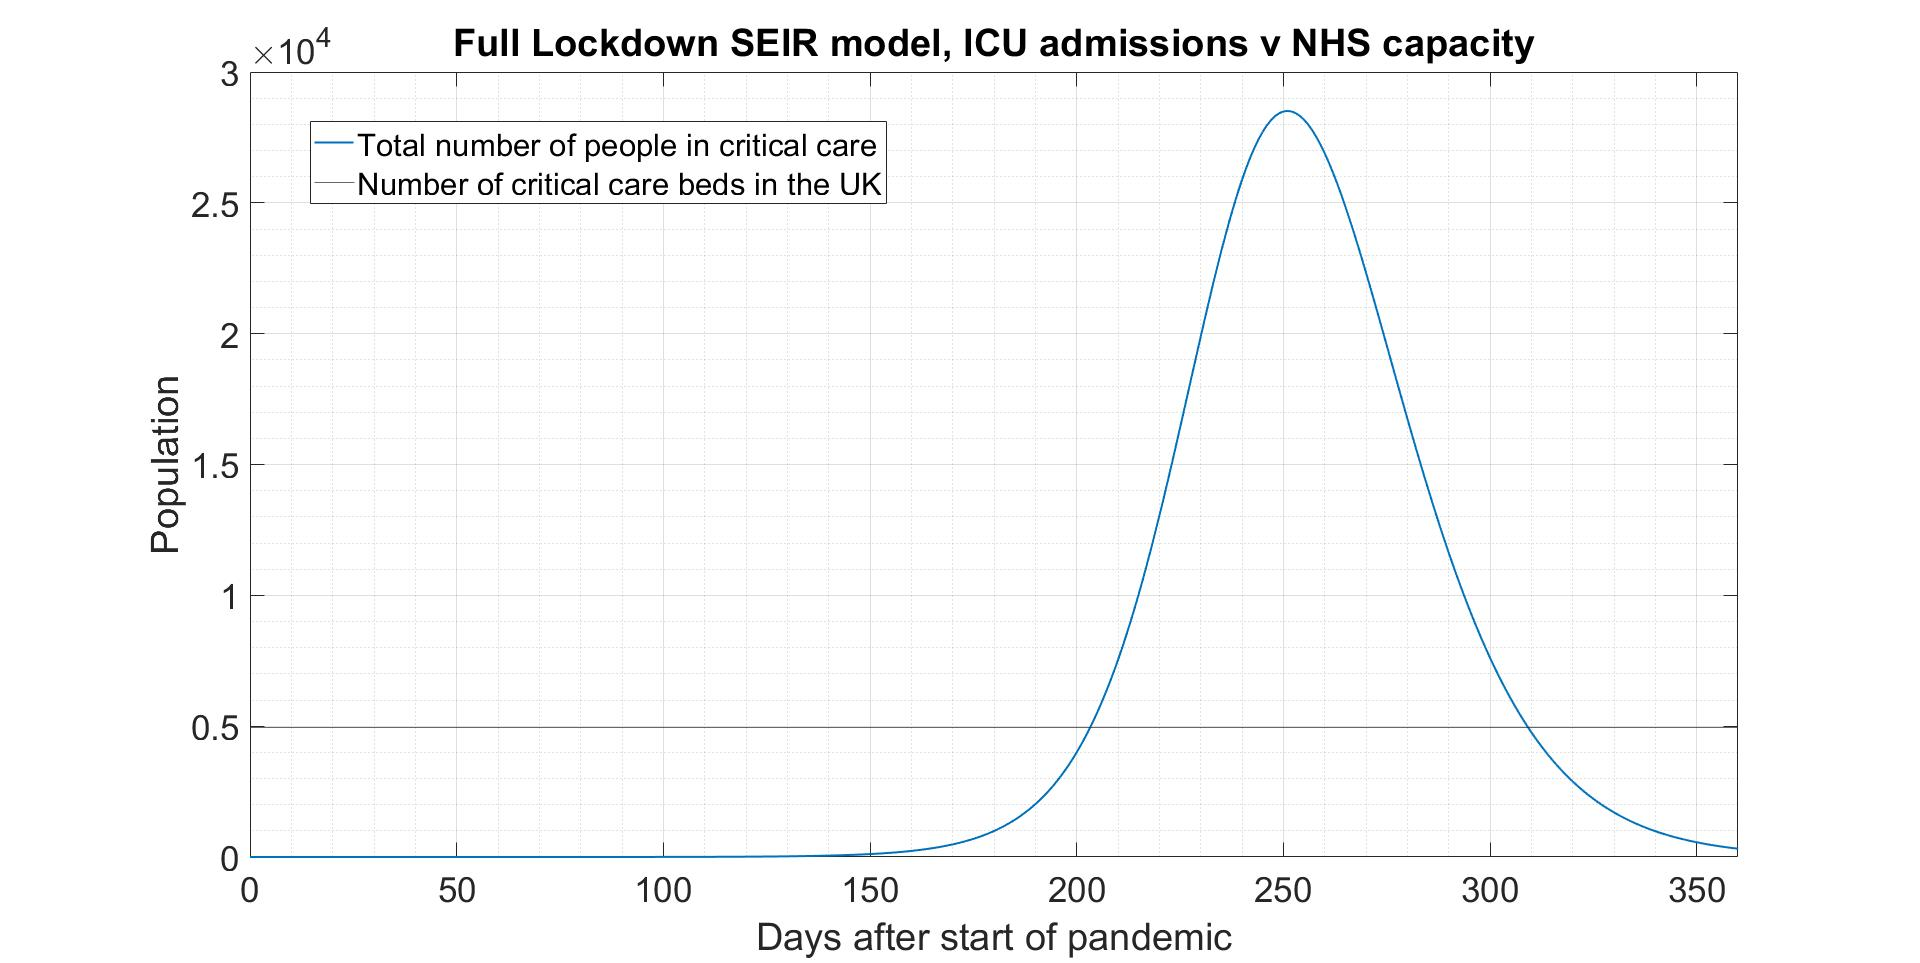
\includegraphics[width=1\textwidth]{FLHICU.jpg} 
\end{center}
Parameters: $R_0=1.085$, $\alpha_1=\frac{2R_0}{7N}$, $\alpha_2=\frac{2R_0}{8.4N}$, $\alpha_3=\frac{2R_0}{12.4N}$, $\gamma_1=\frac{19493-18855}{51279}$, $\gamma_2=\frac{3247-3162}{19493}$ where N is the population of the UK. The peak of infections occurs on day $234$ of the pandemic with $I=6146690$, the peak of hospitalisations occurs on day $241$ of the pandemic with $H=584786$, and the peak of ICU patients occurs on day $251$ with $H_{ICU}=28513$. \par 
The hospitalisations are over capacity from day $203$ to day $282$, for $79$ days, peak over capacity when there are $421850$ more hospitalised people than beds available. The ICU is over capacity from day $204$ to day $309$, which is $105$ days over capacity, peak over capacity when there are $23557$ more people in the ICU than critical care beds available. \par
As mentioned in the analysis of the no-policy environment, the endemic occurs when $\frac{dI}{dt}=0$, hence infections begin to decrease after day $234$. However, the end of all infections occurs on day $508$ with $S=11030000$ and $R=56860000$, R being the number of people immune at the end of infections.
\subsection{Rule of Six}
\begin{center}
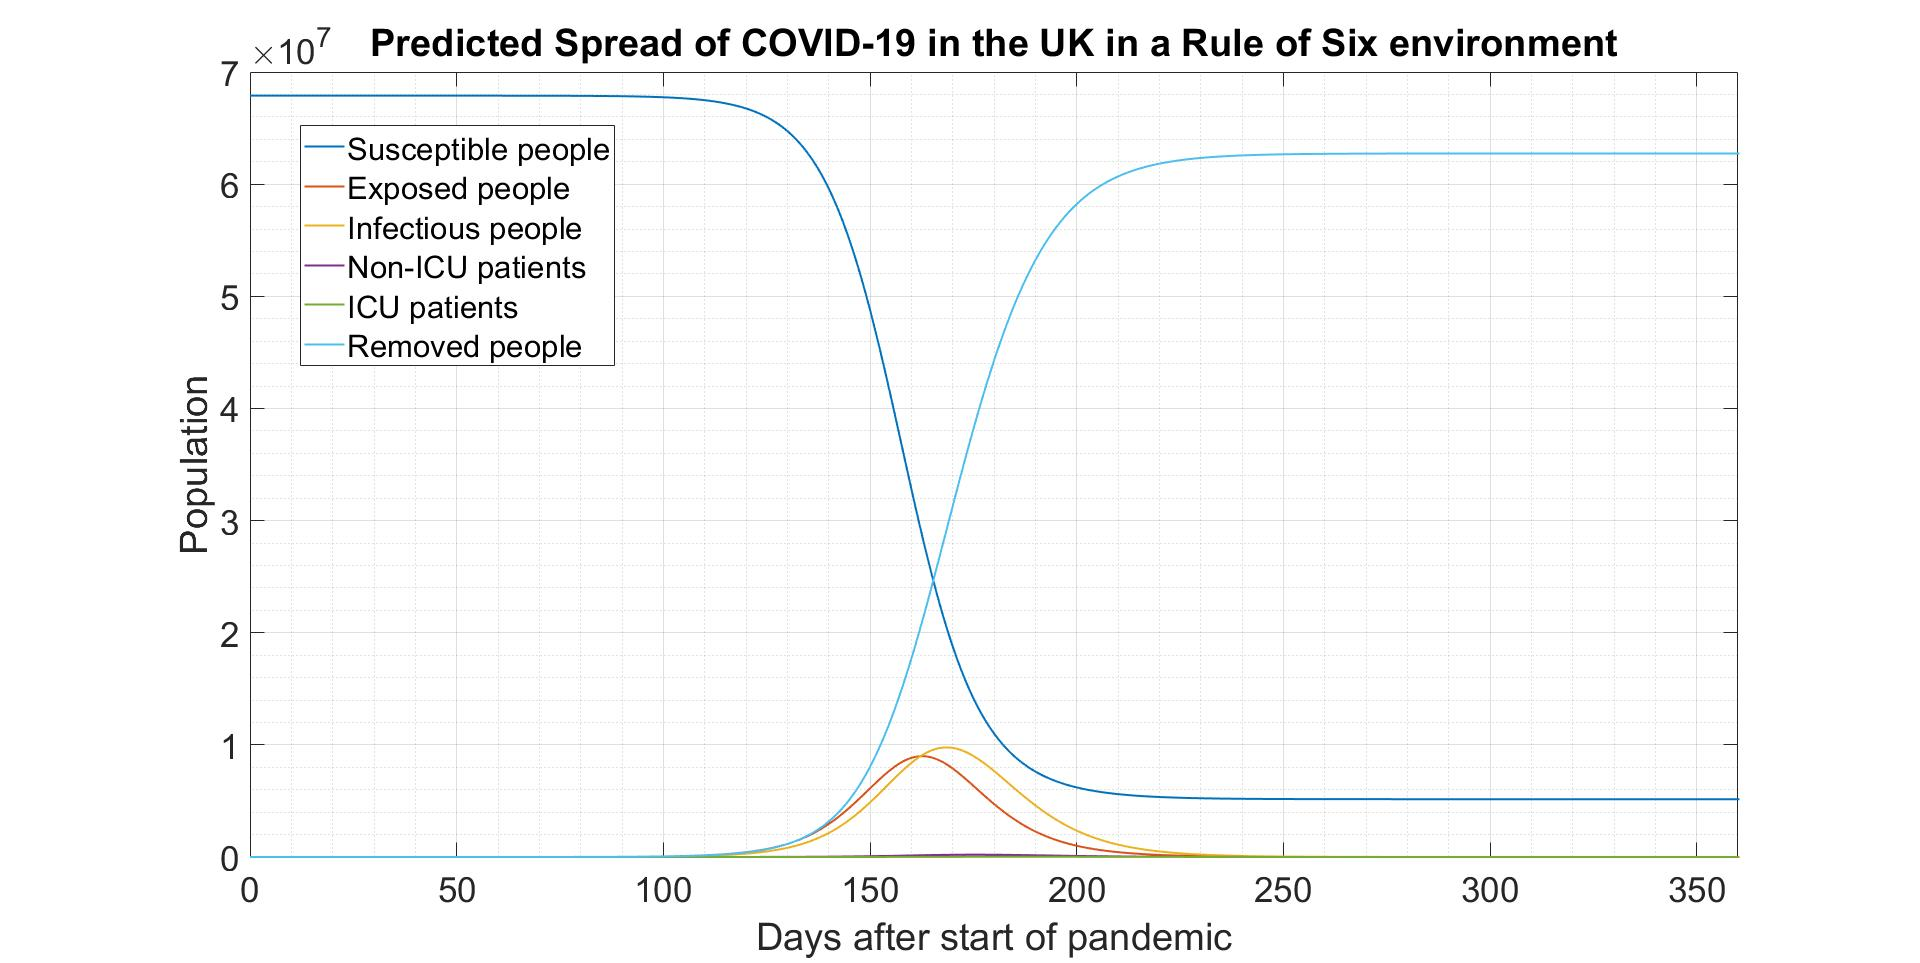
\includegraphics[width=1\textwidth]{ROSSEIHR.jpg} 

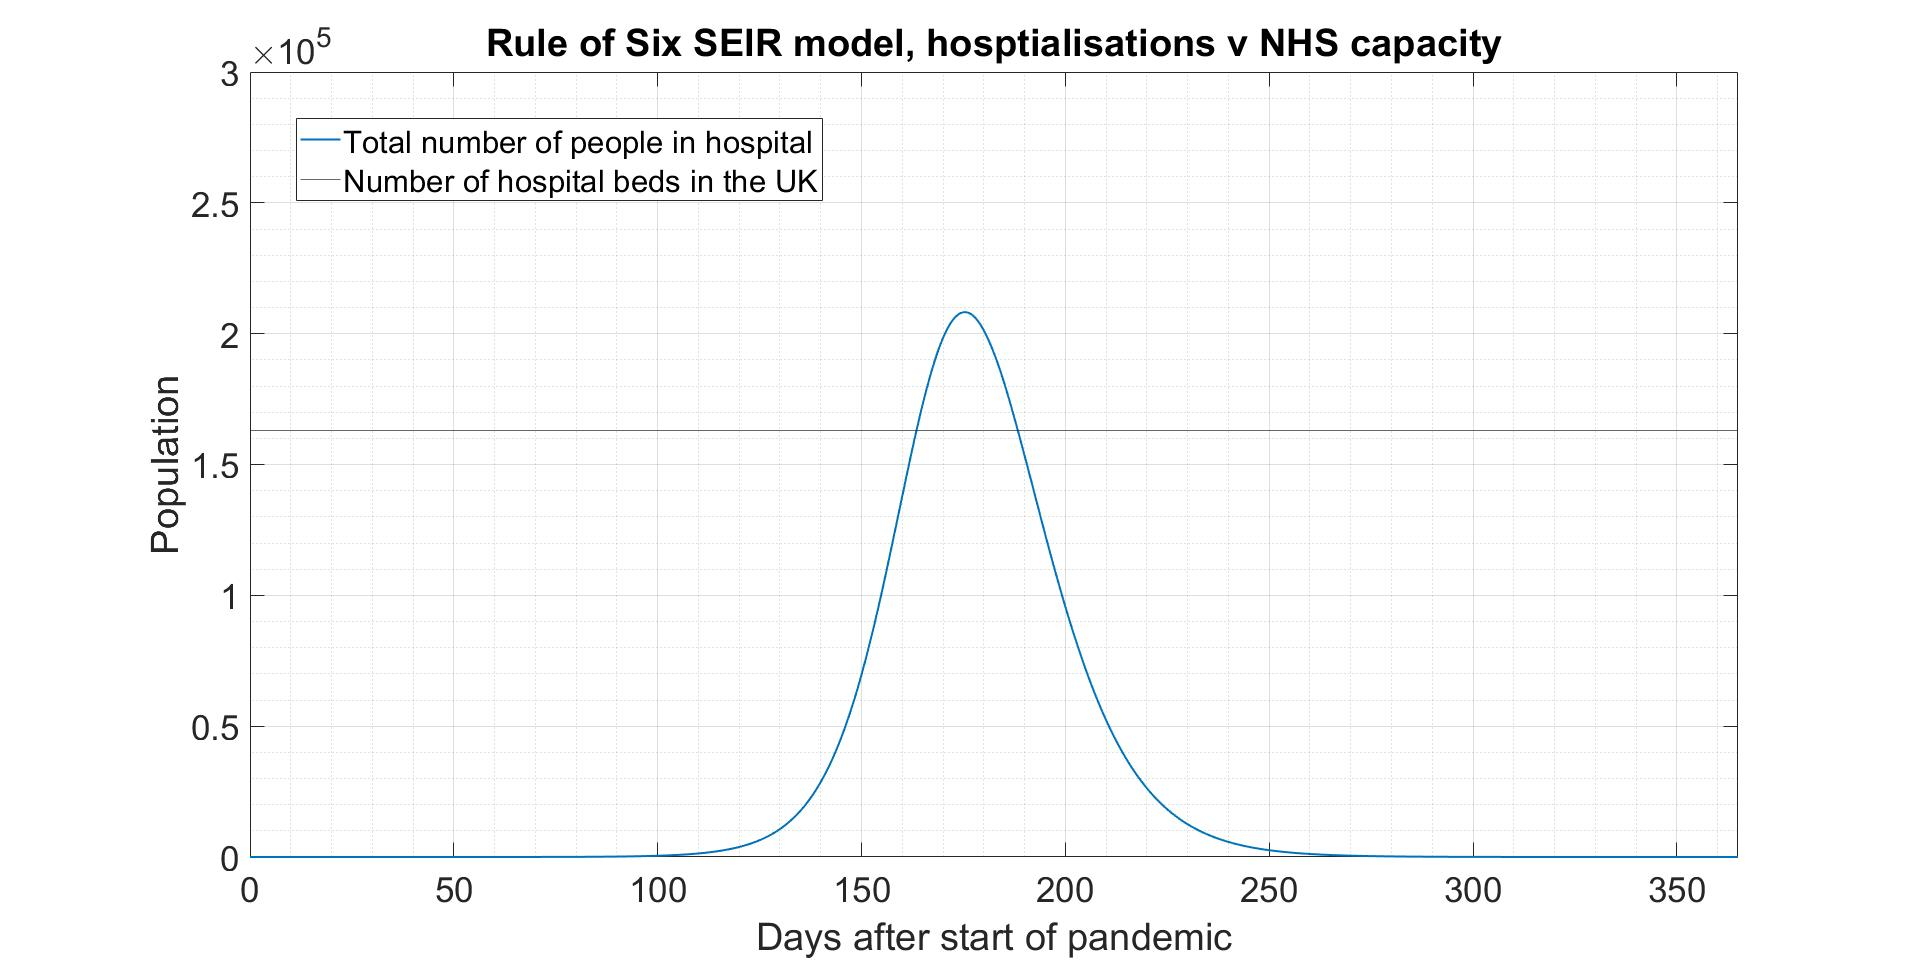
\includegraphics[width=1\textwidth]{ROSH.jpg} 

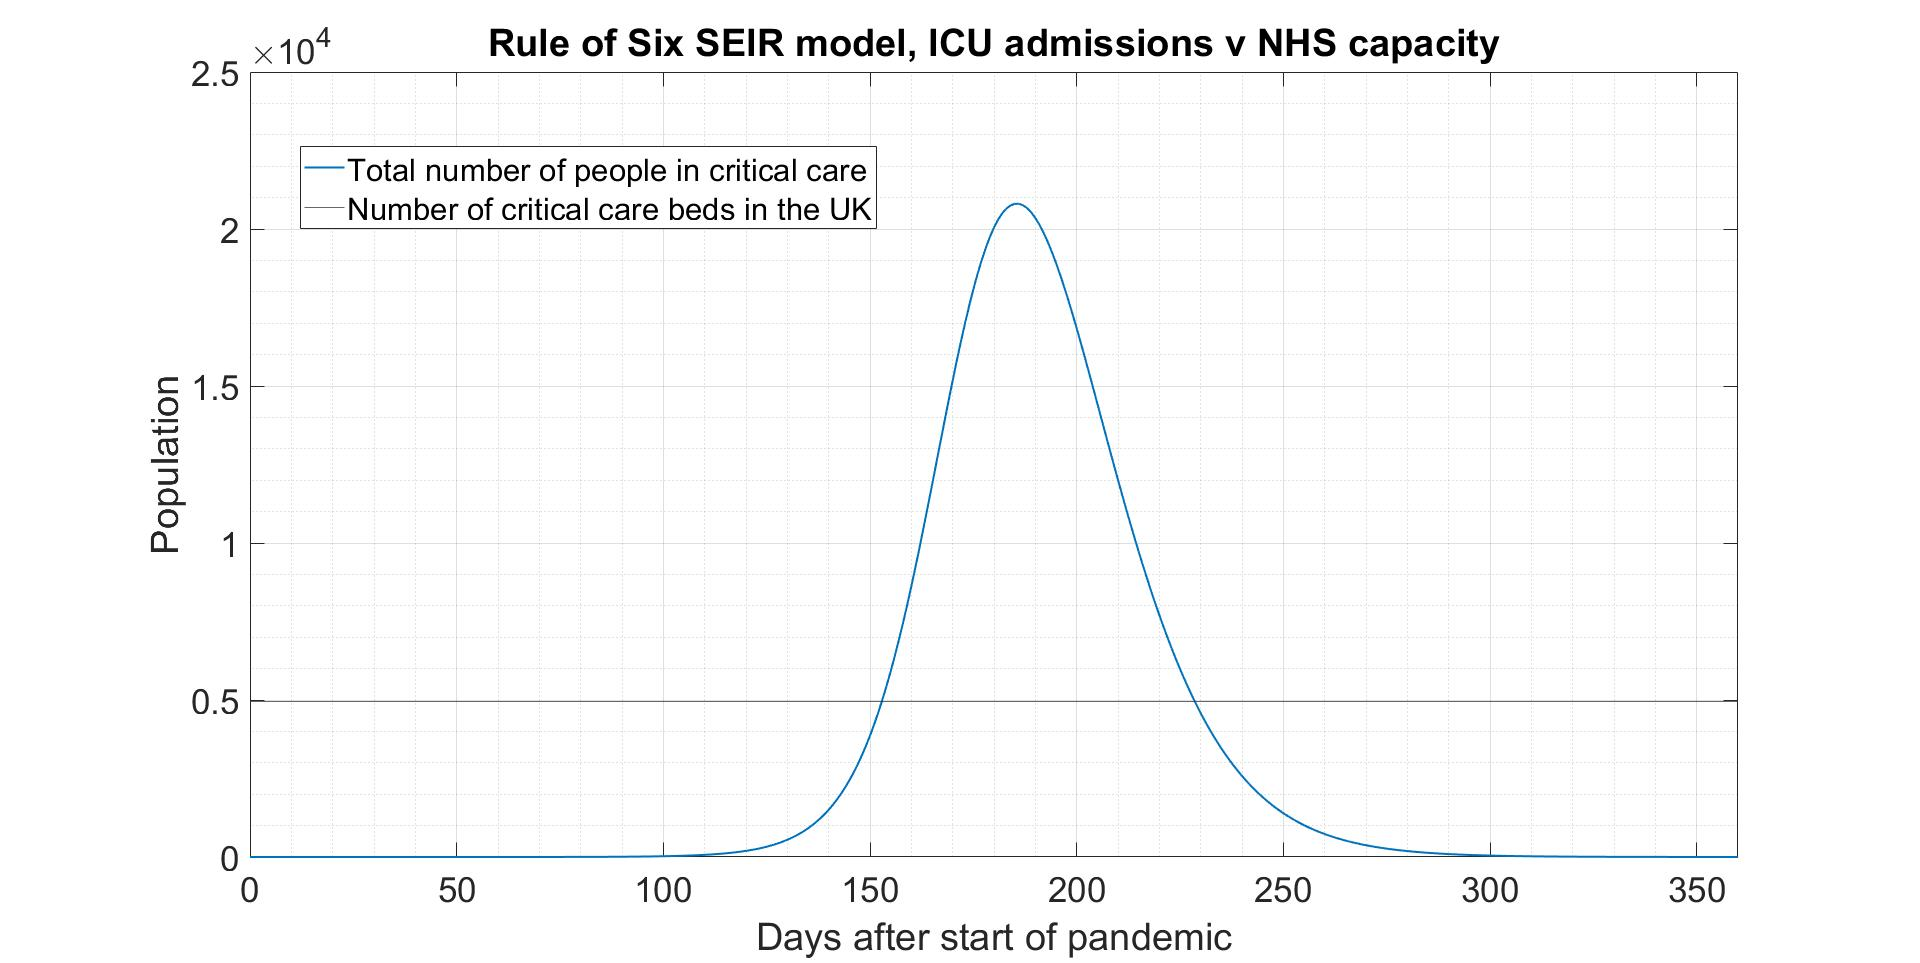
\includegraphics[width=1\textwidth]{ROSHICU.jpg} 
\end{center}
Parameters: $R_0=1.395$, $\alpha_1=\frac{2R_0}{7N}$, $\alpha_2=\frac{2R_0}{8.4N}$, $\alpha_3=\frac{2R_0}{12.4N}$, $\gamma_1=\frac{2020-1846}{58085}$, $\gamma_2=\frac{262-243}{2020}$ where N is the population of the UK. The peak of infections occurs on day $169$ of the pandemic with $I=9766430$, the peak of hospitalisations occurs on day $175$ of the pandemic with $H=208253$, and the peak of ICU patients occurs on day $185$ with $H_{ICU}=20801$. \par 
The hospitalisations are over capacity from day $164$ to day $188$, for $24$ days, peak over capacity when there are $45317$ more hospitalised people than beds available. The ICU is over capacity from day $153$ to day $228$ which is $75$ over capacity, peak over capacity when there are $ 15845$ more people in the ICU than critical care beds available. \par
The endemic occurs on day $169$. However, the end of all infections occurs on day $381$ with $S=5153000$ and $R=62740000$, R being the number of people immune at the end of infections.
\subsection{Local Lockdowns}
\begin{center}
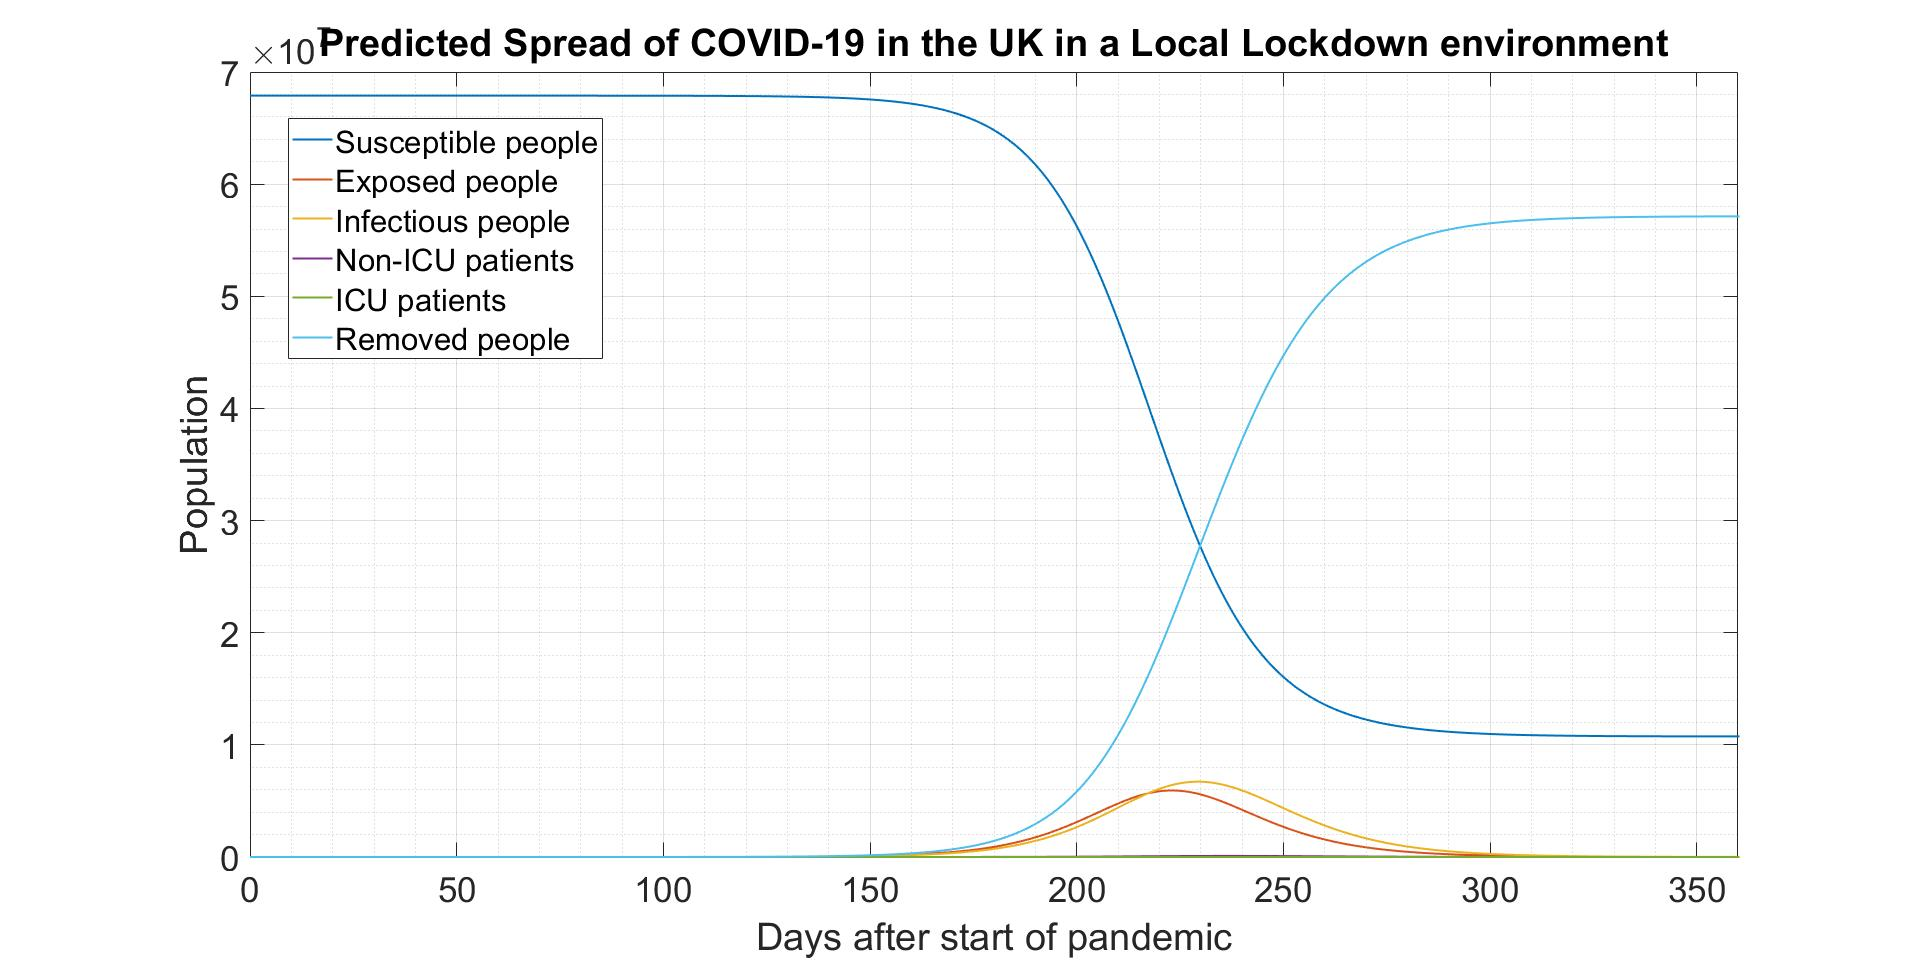
\includegraphics[width=1\textwidth]{LLSEIHR.jpg} 

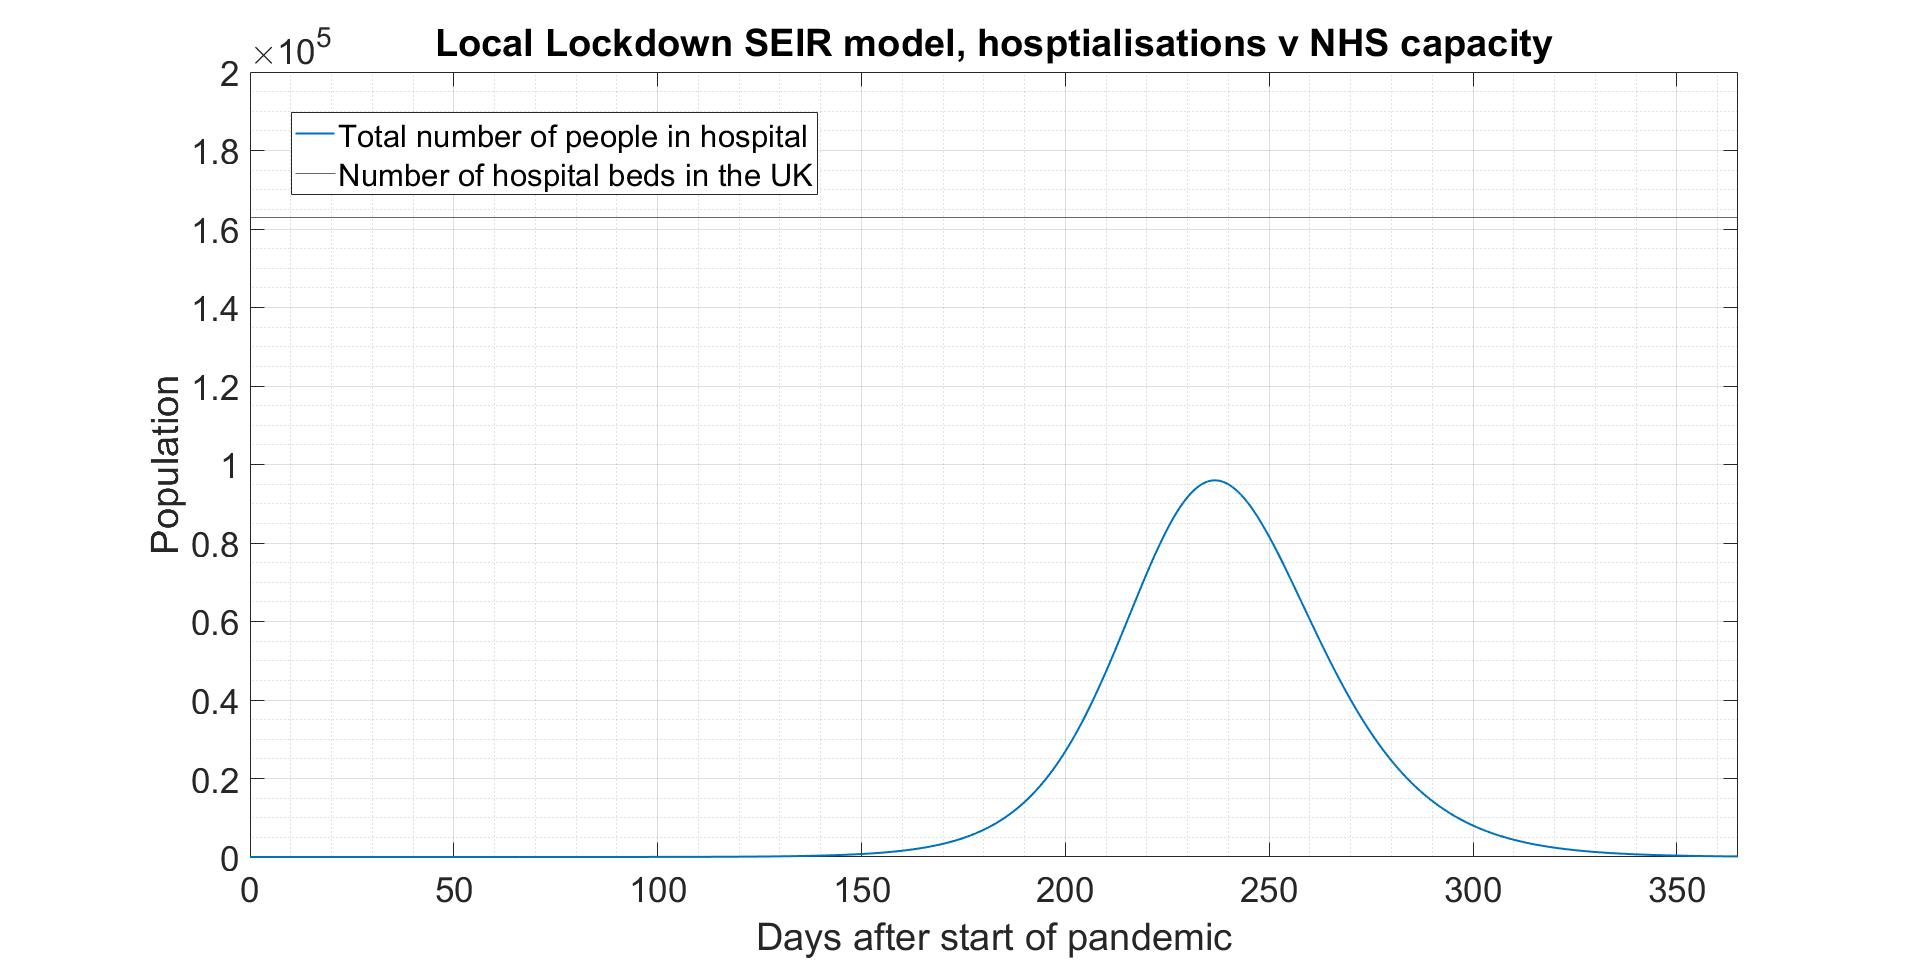
\includegraphics[width=1\textwidth]{LLH.jpg} 

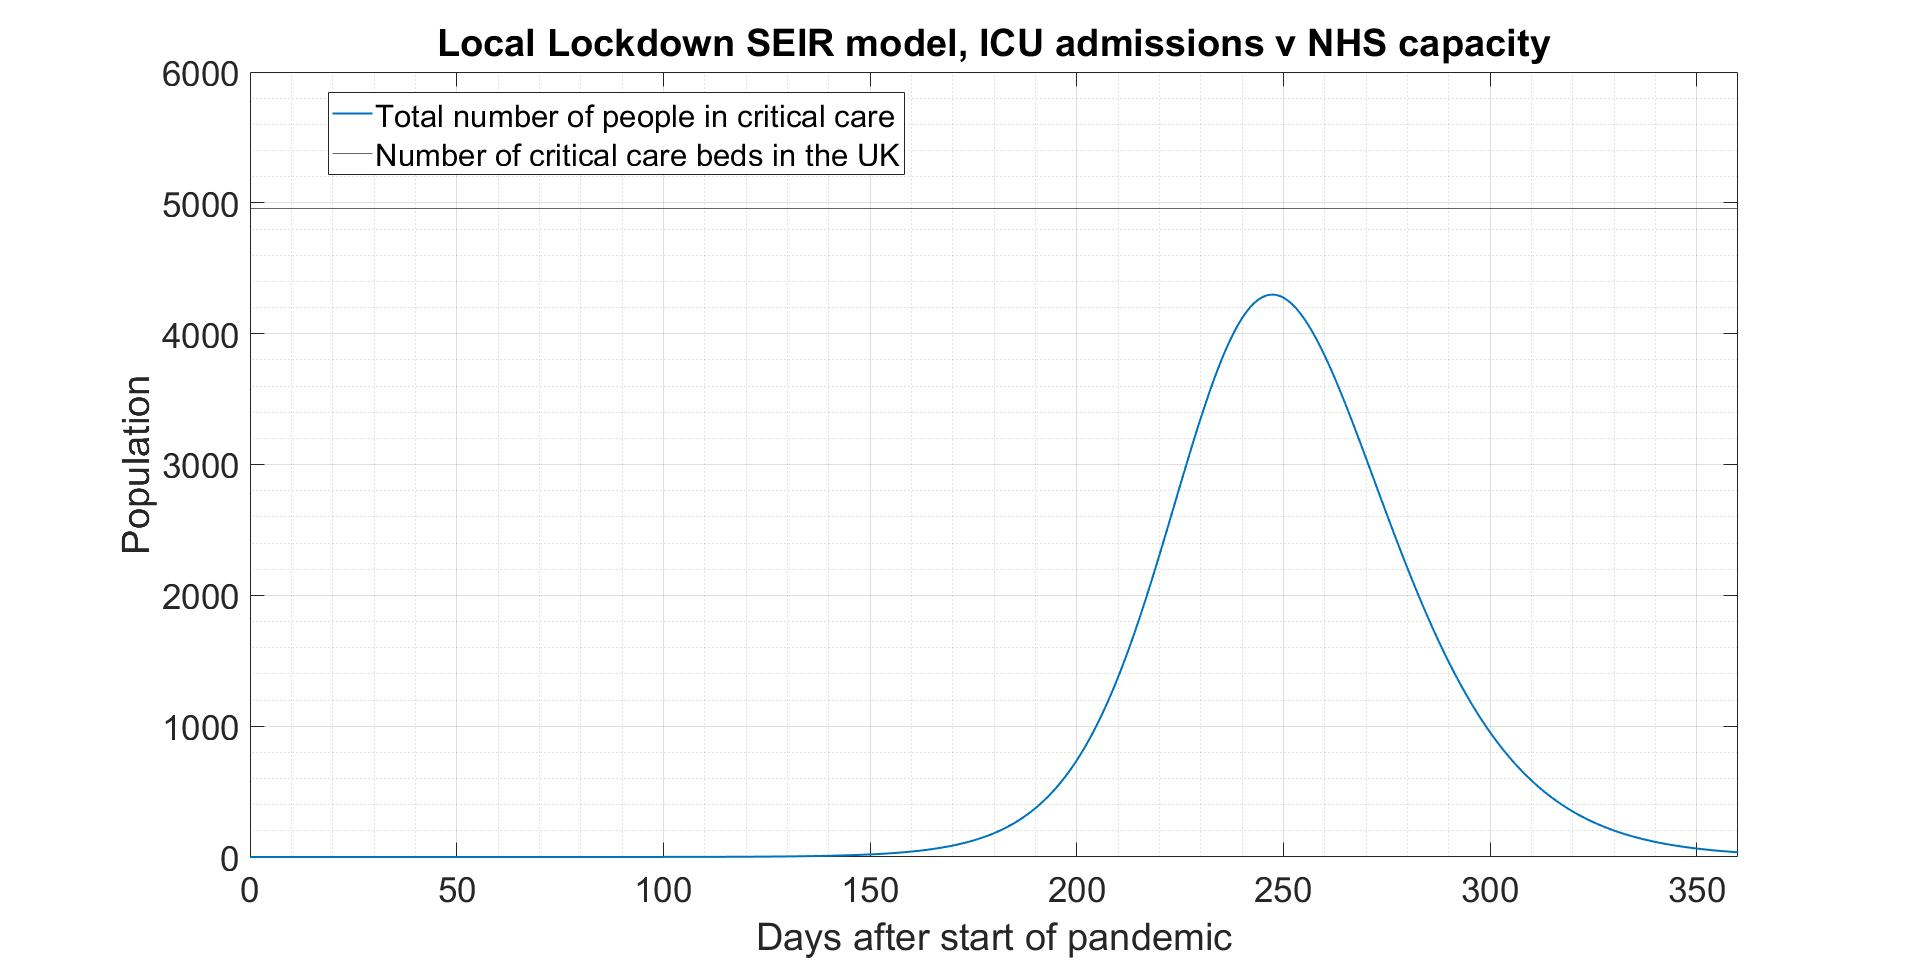
\includegraphics[width=1\textwidth]{LLHICU.jpg} 
\end{center}
Parameters: $R_0=1.095$, $\alpha_1=\frac{2R_0}{7N}$, $\alpha_2=\frac{2R_0}{8.4N}$, $\alpha_3=\frac{2R_0}{12.4N}$, $\gamma_1=\frac{2113-2101}{6428}$, $\gamma_2=\frac{153-145}{1993}$ where N is the population of the UK. The peak of infections occurs on day $230$ of the pandemic with $I=6717240$, the peak of hospitalisations occurs on day $236$ of the pandemic with $H=95933$, and the peak of ICU patients occurs on day $185$ with $H_{ICU}=4298$. \par 
The hospitalisations and ICU cases are always below capacity even at the peak of both. With $67003$ available hospital beds at the peak of hospitalisations and $658$ ICU beds available at the peak of ICU cases. \par
The endemic occurs on day $230$. However, the end of all infections occurs on day $498$ with $S=10750000$ and $R=57140000$, R being the number of people immune at the end of infections.
\subsection{Vaccinations}
A new parameter to consider the proportion of daily vaccinations:
\newline $v$: Rate of vaccinations.
\newline This parameter is calculated using the daily vaccinations over the population of the UK and gives a direct link from susceptible to removed. Creating a new assumption that once vaccinated, immunity follows. Remastered system is given by the following system of ODEs:
\begin{equation}
\begin{aligned}
\frac{dS}{dt}&=- \alpha_1 SI - \alpha_2 SH - \alpha_3 SH_{ICU} - v S \\
\frac{dE}{dt}&= \alpha_1 SI + \alpha_2 SH + \alpha_3 SH_{ICU} - \beta E \\
\frac{dI}{dt}&= \beta E -\gamma_1 I -\delta_1 I \\
\frac{dH}{dt}&= \gamma_1 I - \gamma_2 H -\delta_2 H \\
\frac{dH_{ICU}}{dt}&= \gamma_2 H -\delta_3 H_{ICU} \\
\frac{dR}{dt}&=\delta_1 I + \delta_2 H + \delta_3 H_{ICU} + v S \\
\end{aligned}
\end{equation} 
\begin{center}
\includegraphics[width=1\textwidth]{VSEIHR.jpg} 

\includegraphics[width=1\textwidth]{VH.jpg} 

\includegraphics[width=1\textwidth]{VHICU.jpg} 
\end{center}
Parameters: $R_0=2.4$, $\alpha_1=\frac{2R_0}{7N}$, $\alpha_2=\frac{2R_0}{8.4N}$, $\alpha_3=\frac{2R_0}{12.4N}$, $\gamma_1=\frac{1130-1119}{6428}$, $\gamma_2=\frac{149-144}{1130}$, $v=\frac{485260}{N}$, where $N$ is the population of the UK. The peak of infections occurs on day $136$ of the pandemic with $I=2781110$, the peak of hospitalisations occurs on day $145$ of the pandemic with $H=8348$, and the peak of ICU patients occurs on day $154$ with $H_{ICU}=410$. \par 
The hospitalisations and ICU cases are always below capacity even at the peak of both. With $154588$ available hospital beds at the peak of hospitalisations and $4546$ ICU beds available at the peak of ICU cases. \par
The endemic occurs on day $136$. However, the end of all infections occurs on day $329$ with $S=1429000$ and $R=66460000$, R being the number of people immune at the end of infections.


\section{Conclusion}
\subsection{Limitations}
There are many limitations that come with any model, in fact we can acknowledge that all assumptions lead to limitations. But which of these limitations are significant? This model is data driven; hence the main limitation is the data. To minimise limitations from the data, I used data from only one source\citep{DataSource} for the sake of consistency between different environments I have modelled. All parameters are calculated using data, for no-policy and for strategies, using logic would not allow for comparisons. For example, assuming contact reduced by a half in a full lockdown environment and taking half the no-policy parameters for rate of transmissions would ensure that the lockdown would make a notable change in spread, therefore comparisons will be trivial. \par
Furthermore, using data during the pandemic to model a pandemic from the start will ensure differences in the models that are not due to strategies at the time, however due to which point in time in the pandemic and how much testing is available at said point. We know that COVID-19 is more likely to hospitalise elderly citizens in fact, relative to 18-29 year olds, 50-64 year olds are three times more likely to be hospitalised by COVID-19, and this risk only increases with 85+ year olds ten times more likely to be hospitalised by COVID-19\citep{AGE}. Some parts of the UK, which people may call ‘retirement towns’ have a greater elderly population, and if COVID-19 is currently peaking in said area, then there will be more hospitalisations overall. This is just one of the many reasons why data may not accurately represent strategy effectiveness. Moreover, in these models, I have not considered the existence of variants, which have formed throughout the pandemic, data from later in the pandemic may be affected by this, given some variants have a greater rate of transmission compared to other variants, which again is unrelated to the strategy effectiveness. \par
Other reasons include but are not limited to; lack of people living in accordance with government guidelines, I have assumed that majority of people do comply with assumption $6$ to allow for comparisons, time of the year: Christmas holidays would encourage more people to see families, etc. Again, we must consider limitations due to age, the UK is known for having an elderly population, as mentioned this naturally increases the hospitalisations regardless of effectiveness of strategy. \par
In addition, these models only show one peak, this is due to assumption $7$, For the sake of a simplified model this assumption was necessary, but as we have observed from data this is not the case shown by multiple peaks due to population structure and reinfection. Due to lack of data on the rate of reinfection, I have not included this in my model by assumption $4$. But this does not limit the ability to make comparisons, once we consider these models to display worst case of spread, we can discard the effect on conclusion. \par
Finally in the vaccination environment, we assume that once vaccinated immune, which is true to some extent with most people being protected against serious illness i.e., hospitalisation for approximately six months\citep{WHOVaccine}. My models span over twelve months which may cause hospitalisations to seem less than they are, however if we then assume that within six months people will get their second dose, then this limitation can be discarded.
\subsection{Herd Immunity}
Herd immunity in line with the given models is reached when all the susceptible population is removed, by assumption $3$ ‘All individuals are equally susceptible to COVID-19, and the whole population is considered susceptible at the start of the pandemic’ and assumption $4$ ‘Individuals that are recovered cannot be reinfected i.e., immunity is assumed’ combined implies that once all susceptible people are removed, the whole population is removed and therefore immune. However, we know that this is not the case, since in reality, reinfection is possible, immunity seems to be temporary, and new variants of COVID-19 are continuously being formed due to the global spread. These new variants may be more resistant to immunity hence may be able to infect those who were even more recently infected. For now, vaccines have shown to be effective against all variants so far, hence the spread of vaccines may be the key to herd immunity. \par
In relation to these models herd immunity is given by the steady state of the system $(1)$ and $(2)$:
\begin{equation}
\begin{aligned}
\frac{dS}{dt}&=0\\
\frac{dE}{dt}&= 0 \\
\frac{dI}{dt}&= 0 \\
\frac{dH}{dt}&= 0\\
\frac{dH_{ICU}}{dt}&= 0 \\
\frac{dR}{dt}&=0 \\
\end{aligned}
\end{equation}
The steady state $(3)$ gives an endemic state, there is no change in any variables, and by the one peak model, all differential equations will decrease after this point, hence the pandemic is over. For each model the endemic state will be different as there will be different parameters at play. This is key to comparing strategies as the sooner herd immunity occurs, the sooner the population will return to normality. This should occur at the peak, as any point after the cases are decreasing \par
Since all these peaks happen at different times in the model, solving for $(3)$ is not an easy task. Instead, as I have done when analysing the models, one can consider the point in which infections will start decreasing, this happens at the point: $\frac{dI}{dt}=0$ from this point onwards increasing t will decrease I: $\frac{dI}{dt}<0$. Therefore, this is used as the steady state when analysing. \par
But if we consider the reality of the spread, the spread ‘ends’ when there are no longer any infectious people left, as there is no longer any potential to spread. At this point we have a set of population that is immune, given by the removed category by assumption $4$. In the same way a set of population that has never been infected, given by the susceptible category, but since COVID-19 has been eradicated from system they are no longer at risk, this is when $I<1$.
\subsection{Comparisons}
These models were formed with the goal of comparison; hence these environments represent what the spread would look like if the strategy was implemented from day $1$ of the pandemic. \par
The most successful environments in terms of least infections are as follows:
\begin{enumerate}
\item Vaccination
\item Full Lockdown
\item Local Lockdowns
\item Rule of Six
\item No-policy
\end{enumerate}
The most significant difference is between the vaccination environment and the no-policy environment, with $11201890$ more infections occurring at the peak of no-policy than the vaccination environment. By order of significance, the differences between no policy and strategies are given by $7836310$, $ 7265760$, $ 4216570$; all sufficiently large differences to conclude that a strategy is necessary to contain a pandemic. \par
The most successful environments in terms of least hospitalisations and ICU admissions are as follows:
\begin{enumerate}
\item Vaccination
\item Local Lockdowns
\item Rule of Six
\item Full Lockdown
\item No-policy
\end{enumerate}
Again, the most significant difference is between the vaccination environment and the no-policy environment, with $2674822$ more hospitalisations and $504537$ more ICU cases occurring at the peak of no-policy than the vaccination environment. By order of significance for hospitalisations, the differences between no policy and strategies are given by: $ 2587237$, $ 2474917$, $ 2098384$. In the same way, by the order of significance for ICU cases, the differences are given by: $ 500649$, $ 484146$, $476434$; the differences are of the same order and close in value, meaning all strategies, are approximately equivalent. Again, in terms of NHS capacity, all differences sufficiently large differences to conclude that a strategy is necessary to contain a pandemic. \par
Environments in which hospitalisations and ICU cases were under NHS capacity, in order of most beds available:
\begin{enumerate}
\item Vaccination
\item Local Lockdowns
\end{enumerate}
I have defined $H$ and $H_{ICU}$ for the sake of comparison, in accordance with my project, strategies are only successful if hospitalisations and ICU cases are under NHS capacity. Thus, the only successful strategies are given by the vaccination environment and the local lockdown environment. With the vaccination environment presenting a remarkable difference in beds available for both in general and critical cases, approximately $94.9\%$ hospital beds are available, and $91.7\%$ of ICU beds are available in the no-policy environment. Whereas $41.1\%$ hospital beds are available and $13.3\%$ of ICU beds are available in the local lockdown environment. In the vaccination environment, majority of the hospital beds are available. In contrast, majority of hospital beds are in use in the local lockdown environment. \par
The endemic state for the vaccination environment occurs $ 94$ days before that for the local lockdown environment. Similarly, COVID-19 is eradicated from the vaccination environment system $ 169$ days before the local lockdown environment with $97.9\%$ of the population immune compared to the local lockdown environment that has $84.2\%$ of the population immune. The vaccination environment eradicates COVID-19 from its system at a much earlier date with almost all the population immune, while still maintaining much lower hospitalisations due to COVID-19. Hence, after exhausting all comparative potential, the vaccination environment dominants the local lockdown environment in terms of success.
\subsection{Conclusions}
The no-policy environment is as expected the most unsuccessful environment to tackle a pandemic, out of all the other environments, although the full-lockdown environment is over capacity in terms of hospitalisations for a longer period than the no-policy, the no-policy is the most over capacity by a significantly larger margin which is bound to create more problems than an extra duration of a mere $13$ days. In a no-policy environment, it is guaranteed that there will be an NHS crisis even when taking the model as worst case of spread. Also, no-policy peaked much quicker than any other strategy in turn infections ended much sooner, but at what cost? Hospitals would be hit harder and faster than any other environment since there is less time to gather resources such as PPE to face the pandemic. \par 
The most ideal environment is given by the vaccination environment, by observation flat curves, and lowest peaks in all categories. Hospitalisations and ICU admissions are minimal with most hospital and ICU beds available for other purposes, and with certainty it is the environment least likely to lead to an NHS crisis. \par
As stated in the ‘comparisons’ section, once compared to the no-policy environment, one can see that the differences between strategies are relatively small. But, relative to the NHS capacity i.e., the number of available hospital beds, the smallest differences can be the difference between an NHS crisis and a well contained pandemic. Therefore, the local lockdown environment dominants remaining strategies considering it is below the threshold. The remaining strategies are still effective relative to the no-policy environment, the rule of six environment and full lockdown have the most similarities in hospitalisations. \par
Logically, a full lockdown should reduce the contact much more than the rule of six environment as there is less potential to make physical contact with other households, the similarities in hospitalisation could be due to the fact that the data for full lockdown was taken from earlier in the pandemic, hence more people were immune by the time the rule of six was implemented, a limitation that I have emphasized the importance of: data. Regardless of this, as we have witnessed a full lockdown has long lasting social and economical effects, having this strategy implemented for a full year is unsustainable. The rule of six, is also unsustainable for a year due to the social toll, consequently, strategies should be mixed to allow for sustainability. \par
Local lockdowns are a great alternative to a full lockdown, stopping the spread at its root in a much smaller population easier to control, but when spread is present everywhere these local lockdowns can become a full lockdown. Outlining how strong the vaccination environment is, although it requires much more funding in pandemic research and development of vaccinations, it does pay off once considering its lack of stress on the NHS. A perfect combination of strategies would be to contain spread until vaccinations are available, favouring local lockdowns to keep COVID-19 isolated from the rest of the UK. In order to develop the list of potential strategies, it is important to take note of other successful strategies on a global scale, as in a world of connection and travel, we must tackle global pandemics together to optimize approaches.
\newpage
\bibliography{mybib}
\bibliographystyle{unsrt}
\section{Appendices}
\lstinputlisting[style=Matlab-editor,caption={No-policy environment function with matrix of ODEs} ]{ode_fun_UKcovid.m}
\lstinputlisting[style=Matlab-editor,caption={No-policy environment end of COVID-19 function} ]{findEnd.m}
\lstinputlisting[style=Matlab-editor,caption={No-policy environment using initial data on COVID-19} ]{SEIRMODEL.m}
\begin{verbatim}
COVID-19 is eradicated when, t=270, S=5.816017e+05, R=6.730838e+07
\end{verbatim}

\lstinputlisting[style=Matlab-editor,caption={Vaccination environment function with matrix of ODEs} ]{ode_fun_UKcovidV.m}
\lstinputlisting[style=Matlab-editor,caption={Vaccination environment end of COVID-19 function} ]{findEnd.m}
\lstinputlisting[style=Matlab-editor,caption={Vaccination environment using initial data on COVID-19} ]{SEIRMODELv.m}
\begin{verbatim}
COVID-19 is eradicated when, t=329, S=1.428637e+06, R=6.646136e+07
\end{verbatim}
\end{document}